\SourcePage{137}{140}
\section{Spherical waves}

The plane wave
\[\psi_{\mathbf p}=\operatorname{const}\cdot\exp(i\mathbf p\mathbf r/\hbar)\]
describes a free particle with definite momentum $\mathbf p$ and energy
$E=p^2/2m$. We now consider stationary free-particle states having definite
angular momentum and projection as well as energy. It is convenient to use
the wave vector
\begin{equation}k=\frac p\hbar=\frac{\sqrt{2mE}}\hbar.\tag{33.1}\end{equation}
The state with angular momentum $l$ and projection $m$ has
\begin{equation}\psi_{klm}=R_{kl}(r)Y_{lm}(\theta,\varphi),\tag{33.2}\end{equation}
where
\begin{equation}
 R_{kl}''+\frac2rR_{kl}'+\left[k^2-\frac{l(l+1)}{r^2}\right]R_{kl}=0.\tag{33.3}
\end{equation}
The continuum wave functions satisfy
\[
 \int\psi_{k'l'm'}^*\psi_{klm}dV
 =\delta_{ll'}\delta_{mm'}\delta((k'-k)/2\pi).
\]
Angular functions ensure orthogonality in $l,m$; the radial functions must
\SourcePage{138}{141}
obey
\begin{equation}
 \int_0^\infty r^2R_{k'l}R_{kl}dr=\delta((k'-k)/2\pi)
 =2\pi\delta(k'-k).\tag{33.4}
\end{equation}
For normalization on the energy scale instead,
$\int r^2R_{E'l}R_{El}dr=\delta(E'-E)$, (5.14) gives
\begin{equation}
 R_{El}=R_{kl}\left(\frac1{2\pi}\frac{dk}{dE}\right)^{1/2}
 =\frac1\hbar\sqrt{\frac{m}{2\pi k}}R_{kl}.\tag{33.5}
\end{equation}

For $l=0$, (33.3) reads
$d^2(rR_{k0})/dr^2+k^2rR_{k0}=0$. The finite solution normalized by (33.4)
is
\begin{equation}R_{k0}=2\frac{\sin kr}{r}.\tag{33.6}\end{equation}
For $l\ne0$, put
\begin{equation}R_{kl}=r^l\chi_{kl}.\tag{33.7}\end{equation}
Then
\[\chi_{kl}''+\frac{2(l+1)}r\chi_{kl}'+k^2\chi_{kl}=0.\]
Differentiation gives
\[\chi_{kl}'''+\frac{2(l+1)}r\chi_{kl}''+\left[k^2-\frac{2(l+1)}{r^2}\right]\chi_{kl}'=0.\]
Putting $\chi_{kl}'=r\chi_{k,l+1}$ yields the required equation for
$\chi_{k,l+1}$, so
\begin{equation}\chi_{k,l+1}=\frac1r\chi_{kl}'.\tag{33.8}\end{equation}
\SourcePage{139}{142}
Hence
\[\chi_{kl}=\left(\frac1r\frac d{dr}\right)^l\chi_{k0},\]
where $\chi_{k0}=R_{k0}$ from (33.6), up to an arbitrary constant. Thus
\begin{equation}
 R_{kl}=(-1)^l\,2\frac{r^l}{k^l}\left(\frac1r\frac d{dr}\right)^l\frac{\sin kr}{r}.
 \tag{33.9}
\end{equation}
The factor $k^{-l}$ normalizes the function, and $(-1)^l$ is convenient.
Equivalently,
\begin{equation}
 R_{kl}=\sqrt{\frac{2\pi k}{r}}J_{l+1/2}(kr)=2k j_l(kr),\tag{33.10}
\end{equation}
where the spherical Bessel functions are
\begin{equation}j_l(x)=\sqrt{\frac\pi{2x}}J_{l+1/2}(x).\tag{33.11}\end{equation}
\footnote{The first few are
\[
j_0=\frac{\sin x}x,\quad j_1=\frac{\sin x}{x^2}-\frac{\cos x}x,\quad
j_2=\left(\frac3{x^3}-\frac1x\right)\sin x-\frac{3\cos x}{x^2}.
\]
Another convention in the literature differs from (33.11) by a factor $x$.}

At large $r$, the slowest-decaying term in (33.9) comes from differentiating
the sine $l$ times. Every operation $-d/dr$ shifts its argument by $-\pi/2$,
giving
\begin{equation}R_{kl}\approx\frac2r\sin\left(kr-\frac{\pi l}2\right).\tag{33.12}\end{equation}
Normalization may be performed from the asymptotic form (\secref{21}); comparison
with (33.6) confirms the coefficient in (33.9).
\SourcePage{140}{143}
In the vicinity of the coordinate origin (small $r$), we expand $\sin kr$ in a
series and retain only the term which, after differentiation, produces the
lowest power of $r$\footnote{The symbol $!!$ denotes the product of all numbers
of the same parity up to and including the specified number.}:

\[
\left(\frac1r\frac d{dr}\right)^l\frac{\sin kr}r
\approx\left(\frac1r\frac d{dr}\right)^l\frac{(-1)^l(kr)^{2l+1}}{r(2l+1)!}
=\frac{(-1)^lk^{2l+1}}{(2l+1)!!}.
\]
Therefore
\begin{equation}R_{kl}\approx\frac{2k^{l+1}}{(2l+1)!!}r^l,\tag{33.13}\end{equation}
in agreement with (32.15).

Scattering theory also uses wave functions which are not finite in the usual
sense, but describe particles emitted from or incident on the center. For
$l=0$, replace the standing wave (33.6) by an outgoing or incoming wave:
\begin{equation}R_{k0}^\pm=\frac Ar e^{\pm ikr}.\tag{33.14}\end{equation}
For arbitrary $l$,
\begin{equation}
 R_{kl}^\pm=(-1)^lA\frac{r^l}{k^l}\left(\frac1r\frac d{dr}\right)^l\frac{e^{\pm ikr}}r.
 \tag{33.15}
\end{equation}
In terms of Hankel functions,
\begin{equation}
 R_{kl}^\pm=\pm iA\sqrt{\frac{k\pi}{2r}}H_{l+1/2}^{(1,2)}(kr),\tag{33.16}
\end{equation}
of the first and second kind for $+$ and $-$ respectively. Their asymptotic
forms are
\begin{equation}
 R_{kl}^\pm\approx\frac Ar\exp\left[\pm i\left(kr-\frac{\pi l}2\right)\right],\tag{33.17}
\end{equation}
and near the origin
\begin{equation}R_{kl}^\pm\approx A\frac{(2l-1)!!}{k^l}r^{-l-1}.\tag{33.18}\end{equation}
\SourcePage{141}{144}
Normalize these functions to emission or absorption of one particle per unit
time. Far away, each small part of a spherical wave is locally plane, with
current density $j=v\psi\psi^*$ and $v=k\hbar/m$. The condition
$\oint jdf=1$, or $\int jr^2do=1$, with $do$ the solid-angle element, and the
unchanged angular normalization require
\begin{equation}A=\frac1{\sqrt v}=\sqrt{\frac m{k\hbar}}.\tag{33.19}\end{equation}

An asymptotic expression like (33.12) also holds for positive-energy motion
in any field decreasing sufficiently rapidly with distance.\footnote{It will
be shown in \secref{124} that the field must decrease faster than $1/r$.} At large
$r$, neglecting both the field and centrifugal energy leaves
\[\frac1r\frac{d^2(rR_{kl})}{dr^2}+k^2R_{kl}=0.\]
Its general solution is
\begin{equation}
 R_{kl}\approx2\frac{\sin(kr-l\pi/2+\delta_l)}r,\tag{33.20}
\end{equation}
where $\delta_l$ is the \emph{phase shift}; the coefficient corresponds to
$k/2\pi$ normalization.\footnote{The term $-l\pi/2$ is included so that
$\delta_l=0$ in the absence of a field. Since the overall sign of a wave
function is immaterial, $\delta_l$ is defined modulo $\pi$, not $2\pi$, and
can always be put between 0 and $\pi$.} The exact boundary condition of
finiteness at the origin fixes $\delta_l$. These phases depend on both $l$
and $k$ and are essential characteristics of continuum eigenfunctions.

\ProblemHeading

\textbf{1.} Find the energy levels for $l=0$ motion in the spherical square
well $U(r)=-U_0$ for $r<a$, $U(r)=0$ for $r>a$.
\SourcePage{142}{145}
\SolutionHeading For $l=0$ the wave functions depend only on $r$. Inside,
\[
 \frac1r\frac{d^2}{dr^2}(r\psi)+k^2\psi=0,\qquad
 k=\frac1\hbar\sqrt{2m(U_0-|E|)},
\]
and the finite solution is $\psi=A\sin(kr)/r$. Outside,
\[
 \frac1r\frac{d^2}{dr^2}(r\psi)-\kappa^2\psi=0,\qquad
 \kappa=\frac1\hbar\sqrt{2m|E|},
\]
and the decaying solution is $\psi=A'e^{-\kappa r}/r$. Continuity of the
logarithmic derivative of $r\psi$ at $a$ gives
\begin{equation}
 k\cot ka=-\kappa=-\sqrt{\frac{2mU_0}{\hbar^2}-k^2},\tag{1}
\end{equation}
or
\begin{equation}
 \sin ka=\pm\sqrt{\frac{\hbar^2}{2ma^2U_0}}\,ka.\tag{2}
\end{equation}
These equations implicitly determine the levels, using roots for which
$\cot ka<0$. The first $l=0$ level is also the deepest level of all, the
particle's normal state.

If the well is too shallow, there are no negative-energy levels. Graphically,
the roots of $\pm\sin x=\alpha x$ are intersections of $y=\alpha x$ with
$y=\pm\sin x$, retaining only portions with $\cot x<0$, shown solid in
Fig.~9.

\begin{center}
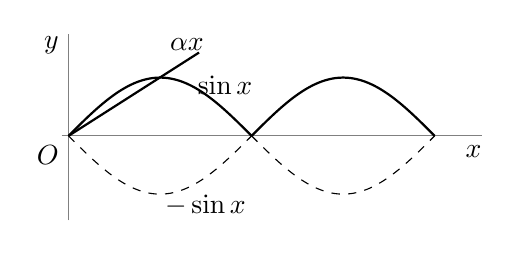
\begin{tikzpicture}[x=0.74cm,y=0.74cm]
 \draw[gray] (0,-1.45)--(0,1.75); \draw[gray] (-0.12,0)--(7.1,0);
 \draw[thick,domain=0:3.1416,samples=80] plot (\x,{sin(\x r)});
 \draw[dashed,domain=3.1416:6.2832,samples=80] plot (\x,{sin(\x r)});
 \draw[dashed,domain=0:3.1416,samples=80] plot (\x,{-sin(\x r)});
 \draw[thick,domain=3.1416:6.2832,samples=80] plot (\x,{-sin(\x r)});
 \draw[thick] (0,0)--(2.24,1.43);
 \node[left] at (0,1.55) {$y$}; \node[below left] at (0,0) {$O$};
 \node[below] at (6.95,0) {$x$}; \node[above] at (2.03,1.29) {$\alpha x$};
 \node[right] at (2.05,0.86) {$\sin x$};
 \node at (2.35,-1.2) {$-\sin x$};
\end{tikzpicture}

\small Fig.~9
\end{center}

For excessive $\alpha$ (small $U_0$) there are no intersections. The first
appears at $\alpha=2/\pi$, $x=\pi/2$. With
$\alpha=\hbar/\sqrt{2ma^2U_0}$ and $x=ka$, the minimum depth is
\begin{equation}U_{0\min}=\frac{\pi^2\hbar^2}{8ma^2}.\tag{3}\end{equation}
It increases as $a$ decreases. At appearance, $ka=\pi/2$ and $E_1=0$.
With further deepening, $E_1$ falls; for small
$\Delta=U_0/U_{0\min}-1$,
\begin{equation}-E_1=(\pi^2/16)U_{0\min}\Delta^2.\tag{4}\end{equation}

\textbf{2.} Find the order of levels with different $l$ in a very deep
spherical well, $U_0\gg\hbar^2/ma^2$ (\emph{W.~Elsasser}, 1933).
\SourcePage{143}{146}
\SolutionHeading As $U_0\to\infty$, the boundary condition is $\psi=0$ at
the wall (\secref{22}). Using (33.10) inside gives
\[J_{l+1/2}(ka)=0.\]
Its roots determine the levels above the well bottom,
$U_0-|E|=\hbar^2k^2/2m$. Starting from the ground state, their order is
\[1s,\ 1p,\ 1d,\ 2s,\ 1f,\ 2p,\ 1g,\ 2d,\ 1h,\ 3s,\ 2f,\ldots\]
The preceding numeral orders levels having the same $l$.\footnote{This
notation is used for particle levels in nuclei (\secref{118}).}

\textbf{3.} Find the order in which levels with different $l$ appear as the
well depth $U_0$ increases.

\SolutionHeading At first appearance a new level has $E=0$. Outside, the
solution vanishing at infinity is $R_l=\operatorname{const}\cdot r^{-(l+1)}$.
Continuity of $R_l,R_l'$ implies
\[(r^{l+1}R_l)'=0\qquad\text{at }r=a.\]
This is equivalent\footnote{From (33.7), (33.8),
$(r^{-l}R_l)'\sim r^{-l}R_{l+1}$. Since (33.3) is invariant under
$l\mapsto-l-1$, also
$(r^{l+1}R_{-l-1})'\sim r^{l+1}R_{-l}$. Since $R_{-l}$ and $R_{l-1}$ obey
the same equation, finally
$(r^{l+1}R_l)'\sim r^{l+1}R_{l-1}$, as used here.} to $R_{l-1}=0$, hence
\[J_{l-1/2}\left(\frac a\hbar\sqrt{2mU_0}\right)=0;\]
for $l=0$, replace $J_{l-1/2}$ by $\cos$. The order of appearance is
\[1s,\ 1p,\ 1d,\ 2s,\ 1f,\ 2p,\ 1g,\ 2d,\ 3s,\ 1h,\ 2f,\ldots\]
Differences from the deep-well ordering begin only for rather high levels.

\textbf{4.} Find the energy levels of the spatial oscillator
$U=\tfrac12m\omega^2r^2$, their degeneracies, and the allowed orbital angular
momenta.

\SolutionHeading Separation in Cartesian coordinates gives three linear
oscillators, hence
\[E=\hbar\omega(n_1+n_2+n_3+3/2)\equiv\hbar\omega(n+3/2).\]
\SourcePage{144}{147}
The degeneracy is the number of ways of writing $n$ as a sum of three
nonnegative integers,\footnote{Equivalently, the number of ways to distribute
$n$ identical balls among three boxes.} namely
\[\frac{(n+1)(n+2)}2.\]
The stationary wave functions are
\begin{equation}
 \psi_{n_1n_2n_3}=\operatorname{const}\cdot e^{-\alpha^2r^2/2}
 H_{n_1}(\alpha x)H_{n_2}(\alpha y)H_{n_3}(\alpha z),\tag{5}
\end{equation}
where $\alpha=\sqrt{m\omega/\hbar}$. Since $H_n$ gains $(-1)^n$ under a
coordinate sign change, (5) has parity $(-1)^n$. Linear combinations at fixed
$n_1+n_2+n_3=n$ yield
\begin{equation}
 \psi_{nlm}=\operatorname{const}\cdot r^le^{-\alpha^2r^2/2}Y_{lm}
 F(-(n-l)/2,l+3/2,\alpha^2r^2),\tag{6}
\end{equation}
where $|m|=0,1,\ldots,l$. The values of $l$ are $0,2,\ldots,n$ for even $n$
and $1,3,\ldots,n$ for odd $n$, as also follows by matching parities
$(-1)^n$ and $(-1)^l$. Thus the level sequence is
\[(1s),\ (1p),\ (1d,2s),\ (1f,2p),\ (1g,2d,3s),\ldots,\]
with mutually degenerate states in parentheses.\footnote{Note the degeneracy
of levels with different $l$; see the note on p.~164.}
